\documentclass[a4paper, 11pt, parskip=half, headsepline]{scrreprt}

\usepackage{scrlayer-scrpage}                   % Headings
\usepackage{txfontsb}                           % Default font
\usepackage{sourcecodepro}                      % Monospace font
\usepackage[utf8]{inputenc}                     % Input encoding
\usepackage[T1]{fontenc}                        % Output encoding
\usepackage{graphicx}                           % Pictures
\usepackage{listings}                           % Code snippets
\usepackage{hyperref}                           % Make strings clickable
% The following commented packages should be already imported by txfontsb
%\usepackage{amsmath,amsfonts,stmaryrd,amssymb} % Math packages
%\usepackage{amsthm}                            % Definitions, theorems, corollaries, ...
%\usepackage{mathtools}                         % Math stuff
\usepackage[usenames,dvipsnames,table]{xcolor}  % Colors
\usepackage[toc,page]{appendix}                 % Support for appendices
\usepackage[chapter]{algorithm}                 % Pseudocode headers
\usepackage{algpseudocode}                      % Pseudocode
\usepackage{pdfpages}                           % Embed external pdf
\usepackage{wrapfig}                            % Wrap text around figures
\usepackage{multicol}                           % Used for multicolumn itemize
\usepackage{multirow}                           % Used for multirow in tables
\usepackage{longtable}                          % Tables can spread over multiple pages
\usepackage{enumerate}                          % Custom item numbers for enumerations
\usepackage[framemethod=tikz]{mdframed}         % Allows defining custom boxed/framed environments
\usepackage{tocloft}                            % TOC spacing




%----------------------------------------------------------------------------------------
%	DOCUMENT SETTINGS
%----------------------------------------------------------------------------------------

\areaset{17cm}{22.5cm}              % Set page width and height
\graphicspath{{./figures/}}         % Set path for figures
\setlength{\cftchapnumwidth}{2em}   % Set chapter numwidth
\setlength{\cftsecnumwidth}{3em}    % Set section numwidth
\setlength{\cftsubsecnumwidth}{4em} % Set subsection numwidth
\hypersetup{linktoc=all}            % Set TOC clickable

\lstset{ 
    belowcaptionskip=\baselineskip,
    aboveskip=\baselineskip,
    breaklines=true,
    frame=l,
    xleftmargin=0.5in,
    showstringspaces=false,
    basicstyle=\footnotesize\ttfamily,
    keywordstyle=\bfseries\color{green!40!black},
    commentstyle=\color{MidnightBlue},
    stringstyle=\color{BrickRed},
    numberstyle=\color{Cyan!50!Black},
    numbers=left,
    tabsize=4
}

\pagestyle{scrheadings}
\ihead{Usability Evaluation Study 1: Inspection}
\ohead{Codiglioni, dell'Oglio, Nichelini}


%----------------------------------------------------------------------------------------
%	COMMAND LINE ENVIRONMENT
%----------------------------------------------------------------------------------------

% Usage:
% \begin{commandline}
%	\begin{verbatim}
%		$ ls
%		
%		Applications	Desktop	...
%	\end{verbatim}
% \end{commandline}

\mdfdefinestyle{commandline}{
	leftmargin=10pt,
	rightmargin=10pt,
	innerleftmargin=15pt,
	middlelinecolor=black!50!white,
	middlelinewidth=2pt,
	frametitlerule=false,
	backgroundcolor=black!5!white,
	frametitle={Command line},
	frametitlefont={\normalfont\ttfamily\color{white}\hspace{-1em}},
	frametitlebackgroundcolor=black!50!white,
	nobreak,
}

% Define a custom environment for command-line snapshots
\newenvironment{commandline}{
	\medskip
	\begin{mdframed}[style=commandline]
	\footnotesize
}{
	\end{mdframed}
	\medskip
}


%----------------------------------------------------------------------------------------
%	FILE CONTENTS ENVIRONMENT
%----------------------------------------------------------------------------------------

% Usage:
% \begin{file}[optional filename, defaults to "File"]
%	File contents, for example, with a listings environment
% \end{file}

\mdfdefinestyle{file}{
	innertopmargin=1.6\baselineskip,
	innerbottommargin=0.28\baselineskip,
	topline=false, bottomline=false,
	leftline=false, rightline=false,
	leftmargin=2cm,
	rightmargin=2cm,
	singleextra={%
		\draw[fill=black!10!white](P)++(0,-1.3em)rectangle(P-|O);
		\node[anchor=north west]
		at(P-|O){\footnotesize\ttfamily\mdfilename};
		%
		\def\l{1.5em}
		\draw(O-|P)++(-\l,0)--++(\l,\l)--(P)--(P-|O)--(O)--cycle;
		\draw(O-|P)++(-\l,0)--++(0,\l)--++(\l,0);
	},
	nobreak,
}

% Define a custom environment for file contents
\newenvironment{file}[1][File]{ % Set the default filename to "File"
	\medskip
	\newcommand{\mdfilename}{#1}
	\begin{mdframed}[style=file]
}{
	\end{mdframed}
	\medskip
}


%----------------------------------------------------------------------------------------
%	NUMBERED QUESTIONS ENVIRONMENT
%----------------------------------------------------------------------------------------

% Usage:
% \begin{question}[optional title]
%	Question contents
% \end{question}

\mdfdefinestyle{question}{
	innertopmargin=1.2\baselineskip,
	innerbottommargin=0.8\baselineskip,
	roundcorner=5pt,
	nobreak,
	singleextra={%
		\draw(P-|O)node[xshift=1em,anchor=west,fill=white,draw,rounded corners=5pt]{%
		Question \theQuestion\questionTitle};
	},
}

\newcounter{Question} % Stores the current question number that gets iterated with each new question

% Define a custom environment for numbered questions
\newenvironment{question}[1][\unskip]{
	\bigskip
	\stepcounter{Question}
	\newcommand{\questionTitle}{~#1}
	\begin{mdframed}[style=question]
}{
	\end{mdframed}
	\medskip
}


%----------------------------------------------------------------------------------------
%	BOXED PARAGRAPH ENVIRONMENT
%----------------------------------------------------------------------------------------

% Usage:
% \begin{boxedpar}[optional title]
%	Question contents
% \end{boxedpar}

\mdfdefinestyle{boxedpar}{
	innertopmargin=1.2\baselineskip,
	innerbottommargin=0.8\baselineskip,
	roundcorner=5pt,
	nobreak,
	singleextra={%
		\draw(P-|O)node[xshift=1em,anchor=west,fill=white,draw,rounded corners=5pt]{%
		\textit{\boxTitle}};
	},
}

% Define a custom environment for numbered questions
\newenvironment{boxedpar}[1][in-depth]{
	\bigskip
	\newcommand{\boxTitle}{#1}
	\begin{mdframed}[style=boxedpar]
}{
	\end{mdframed}
	\medskip
}


%----------------------------------------------------------------------------------------
%	ROUNDED BOX ENVIRONMENT
%----------------------------------------------------------------------------------------

% Usage:
% \begin{roundedbox}
%	Contents
% \end{roundedbox}

\mdfdefinestyle{roundedbox}{
	innertopmargin=0.5\baselineskip,
	innerbottommargin=0.5\baselineskip,
	roundcorner=5pt,
	nobreak,
}

% Define a custom environment for numbered questions
\newenvironment{roundedbox}{
	\bigskip
	\begin{mdframed}[style=roundedbox]
}{
	\end{mdframed}
	\medskip
}


%----------------------------------------------------------------------------------------
%	WARNING TEXT ENVIRONMENT
%----------------------------------------------------------------------------------------

% Usage:
% \begin{warn}[optional title, defaults to "Warning:"]
%	Contents
% \end{warn}

\mdfdefinestyle{warning}{
	topline=false, bottomline=false,
	leftline=false, rightline=false,
	nobreak,
	singleextra={%
		\draw(P-|O)++(-0.5em,0)node(tmp1){};
		\draw(P-|O)++(0.5em,0)node(tmp2){};
		\fill[black,rotate around={45:(P-|O)}](tmp1)rectangle(tmp2);
		\node at(P-|O){\color{white}\scriptsize\textbf !};
		\draw[very thick](P-|O)++(0,-1em)--(O);%--(O-|P);
	}
}

% Define a custom environment for warning text
\newenvironment{warn}[1][Warning:]{ % Set the default warning to "Warning:"
	\medskip
	\begin{mdframed}[style=warning]
		\noindent{\textbf{#1}}
}{
	\end{mdframed}
}


%----------------------------------------------------------------------------------------
%	INFORMATION ENVIRONMENT
%----------------------------------------------------------------------------------------

% Usage:
% \begin{info}[optional title, defaults to "Info:"]
% 	contents
% 	\end{info}

\mdfdefinestyle{info}{%
	topline=false, bottomline=false,
	leftline=false, rightline=false,
	nobreak,
	singleextra={%
		\fill[black](P-|O)circle[radius=0.4em];
		\node at(P-|O){\color{white}\scriptsize\textbf i};
		\draw[very thick](P-|O)++(0,-0.8em)--(O);%--(O-|P);
	}
}

% Define a custom environment for information
\newenvironment{info}[1][Info:]{ % Set the default title to "Info:"
	\medskip
	\begin{mdframed}[style=info]
		\noindent{\textbf{#1}}
}{
	\end{mdframed}
}


%----------------------------------------------------------------------------------------
%	LINEDQUOTE ENVIRONMENT
%----------------------------------------------------------------------------------------

% Usage:
% \begin{linedquote}
% 	contents
% 	\end{linedquote}

\mdfdefinestyle{linedquote}{%
	topline=false, bottomline=false,
	leftline=false, rightline=false,
	nobreak,
	singleextra={%
		\draw[very thick](P-|O)++(0,0)--(O);%--(O-|P);
	}
}

% Define a custom environment
\newenvironment{linedquote}{
	\begin{mdframed}[style=linedquote]
}{
	\end{mdframed}
}


%----------------------------------------------------------------------------------------
%	TITLE PAGE
%----------------------------------------------------------------------------------------

\title{Usability Evaluation Study 1:\\ Inspection }
\subtitle{\href{https://www.visitmonterosa.com}{www.visitmonterosa.com}}
\author{Fabio Codiglioni - 10484720\\fabio.codiglioni@mail.polimi.it\\\\Luca dell'Oglio - 10497928\\luca1.delloglio@mail.polimi.it\\\\Alessandro Nichelini - 10497404\\alessandro.nichelini@mail.polimi.it}
\date{March 25$^{th}$, 2020}
\publishers{
    \begin{figure}[t]
        \centering
        
\includegraphics[width=0.5\linewidth, keepaspectratio]{Logo_Politecnico_Milano}
    \end{figure}
}


%----------------------------------------------------------------------------------------
%	DOCUMENT
%----------------------------------------------------------------------------------------

\begin{document}

% Title page and TOC
\pagenumbering{gobble}
\maketitle
%\shipout\null           % Blank page
\pagenumbering{roman}
\tableofcontents
\newpage
\pagenumbering{arabic}

% Body

\chapter{Introduction}

% TODO: Todo

\chapter{Heuristic evaluation}

\begin{center}
    \def\arraystretch{1.3}
    \begin{tabular}{|l|l|c|c|c|c|}
        \hline
        \textbf{Category} & \textbf{Heuristics} & \textbf{Codiglioni} & \textbf{dell'Oglio} & \textbf{Nichelini} & \textbf{Total score} \\ \hline
        \multirow{5}{*}{\textit{Navigation}} & Interaction consistency & 3 & 4 & 3 & 3 \\ \cline{2-6}
        & Group navigation & 3 & 3 & 2 & 2 \\ \cline{2-6}
        & Structural navigation & 5 & 5 & 5 & 5 \\ \cline{2-6}    % TODO
        & Semantic navigation & 4 & 3 & 3 & 3 \\ \cline{2-6}
        & Landmarks & 5 & 4 & 5 & 5 \\ \hline
        \multirow{1}{*}{\textit{Content}} & Information overload & 5 & 5 & 4 & 5 \\ \hline
        \multirow{4}{*}{\textit{Layout}} & Text layout & 4 & 5 & 4 & 4 \\ \cline{2-6}
        & Interaction placeholder & 4 & 3 & 3 & 3 \\ \cline{2-6}
        & Spatial allocation & 5 & 4 & 3 & 4 \\ \cline{2-6}
        & Consistency of page structure & 4 & 5 & 5 & 5 \\ \hline
    \end{tabular}
\end{center}

% TODO: Screenshots 1-3:    Fabio
% TODO: Screenshots 4-7:    Ale
% TODO: Screenshots 8-10:   Luca

\section{Navigation}

\paragraph{Interaction consistency}
\begin{itemize}
    \item Link structure is consistent. % TODO
    \item When you click on entries under "Experience Monterosa", some of these have a suggestions section, others do not (Figures \ref{fig:interaction-consistency-01} and \ref{fig:interaction-consistency-02}).
    \item The entries shown when you click "Experience Monterosa" are different than the ones shown in the drop-down menu. In general, you cannot always reach 2nd level entries once you clicked on 1st level ones (Figures \ref{fig:interaction-consistency-03} and \ref{fig:interaction-consistency-04}).
    \item "Eventi" has no drop-down menu.
    \item The same links have different labels based on "Inverno"/"Estate" (Figures \ref{fig:interaction-consistency-05} and \ref{fig:interaction-consistency-06}).
\end{itemize}

\begin{figure}[H]
    \begin{minipage}[t]{0.5\textwidth}
        \centering
        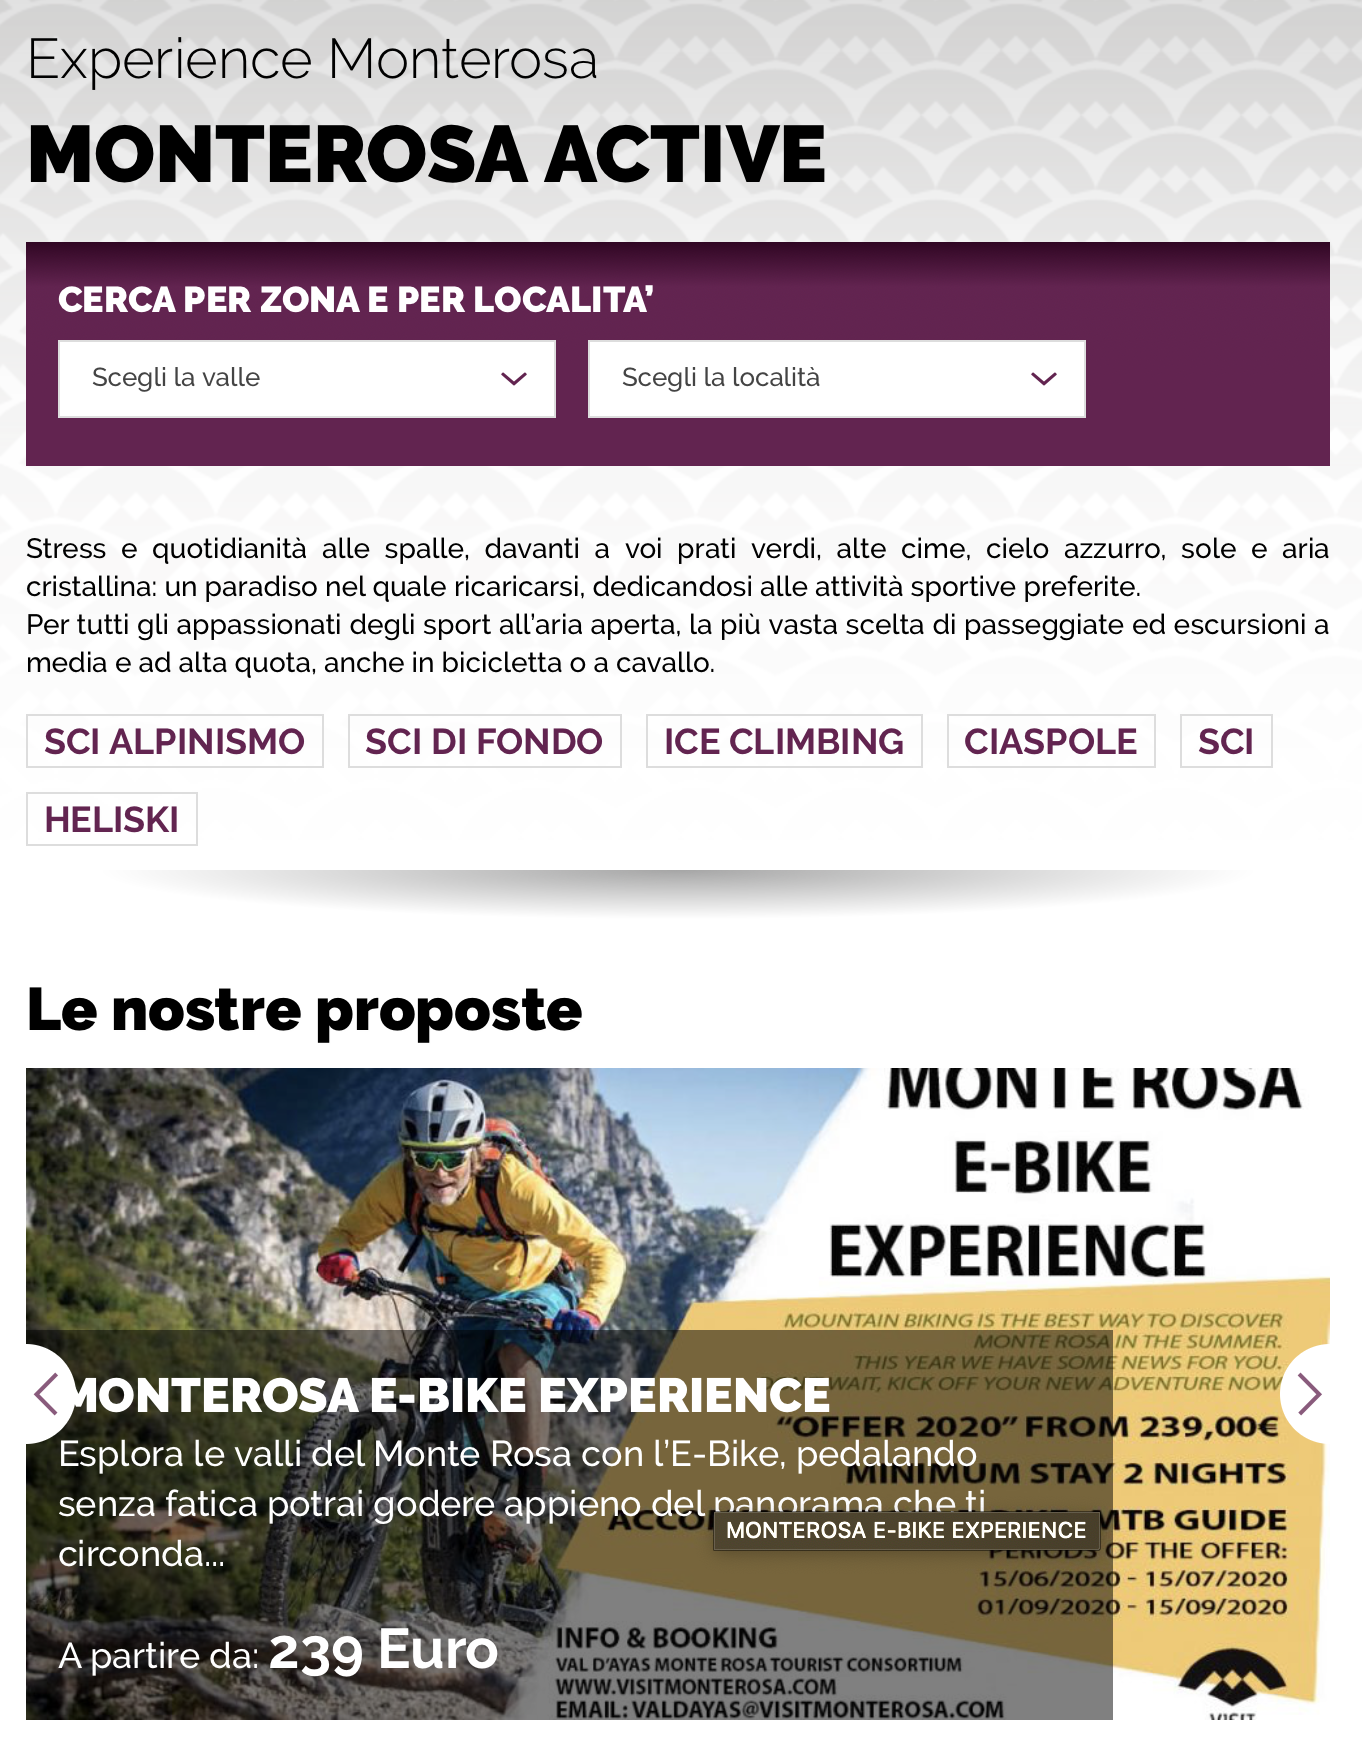
\includegraphics[width=1\linewidth, keepaspectratio]{11-interaction-consistency}
        \caption{\href{https://www.visitmonterosa.com/experience-monterosa/monterosa-active/}{link}.}
        \label{fig:interaction-consistency-01}
    \end{minipage}   
    \hspace*{\fill}
    \begin{minipage}[t]{0.5\textwidth}
        \centering
        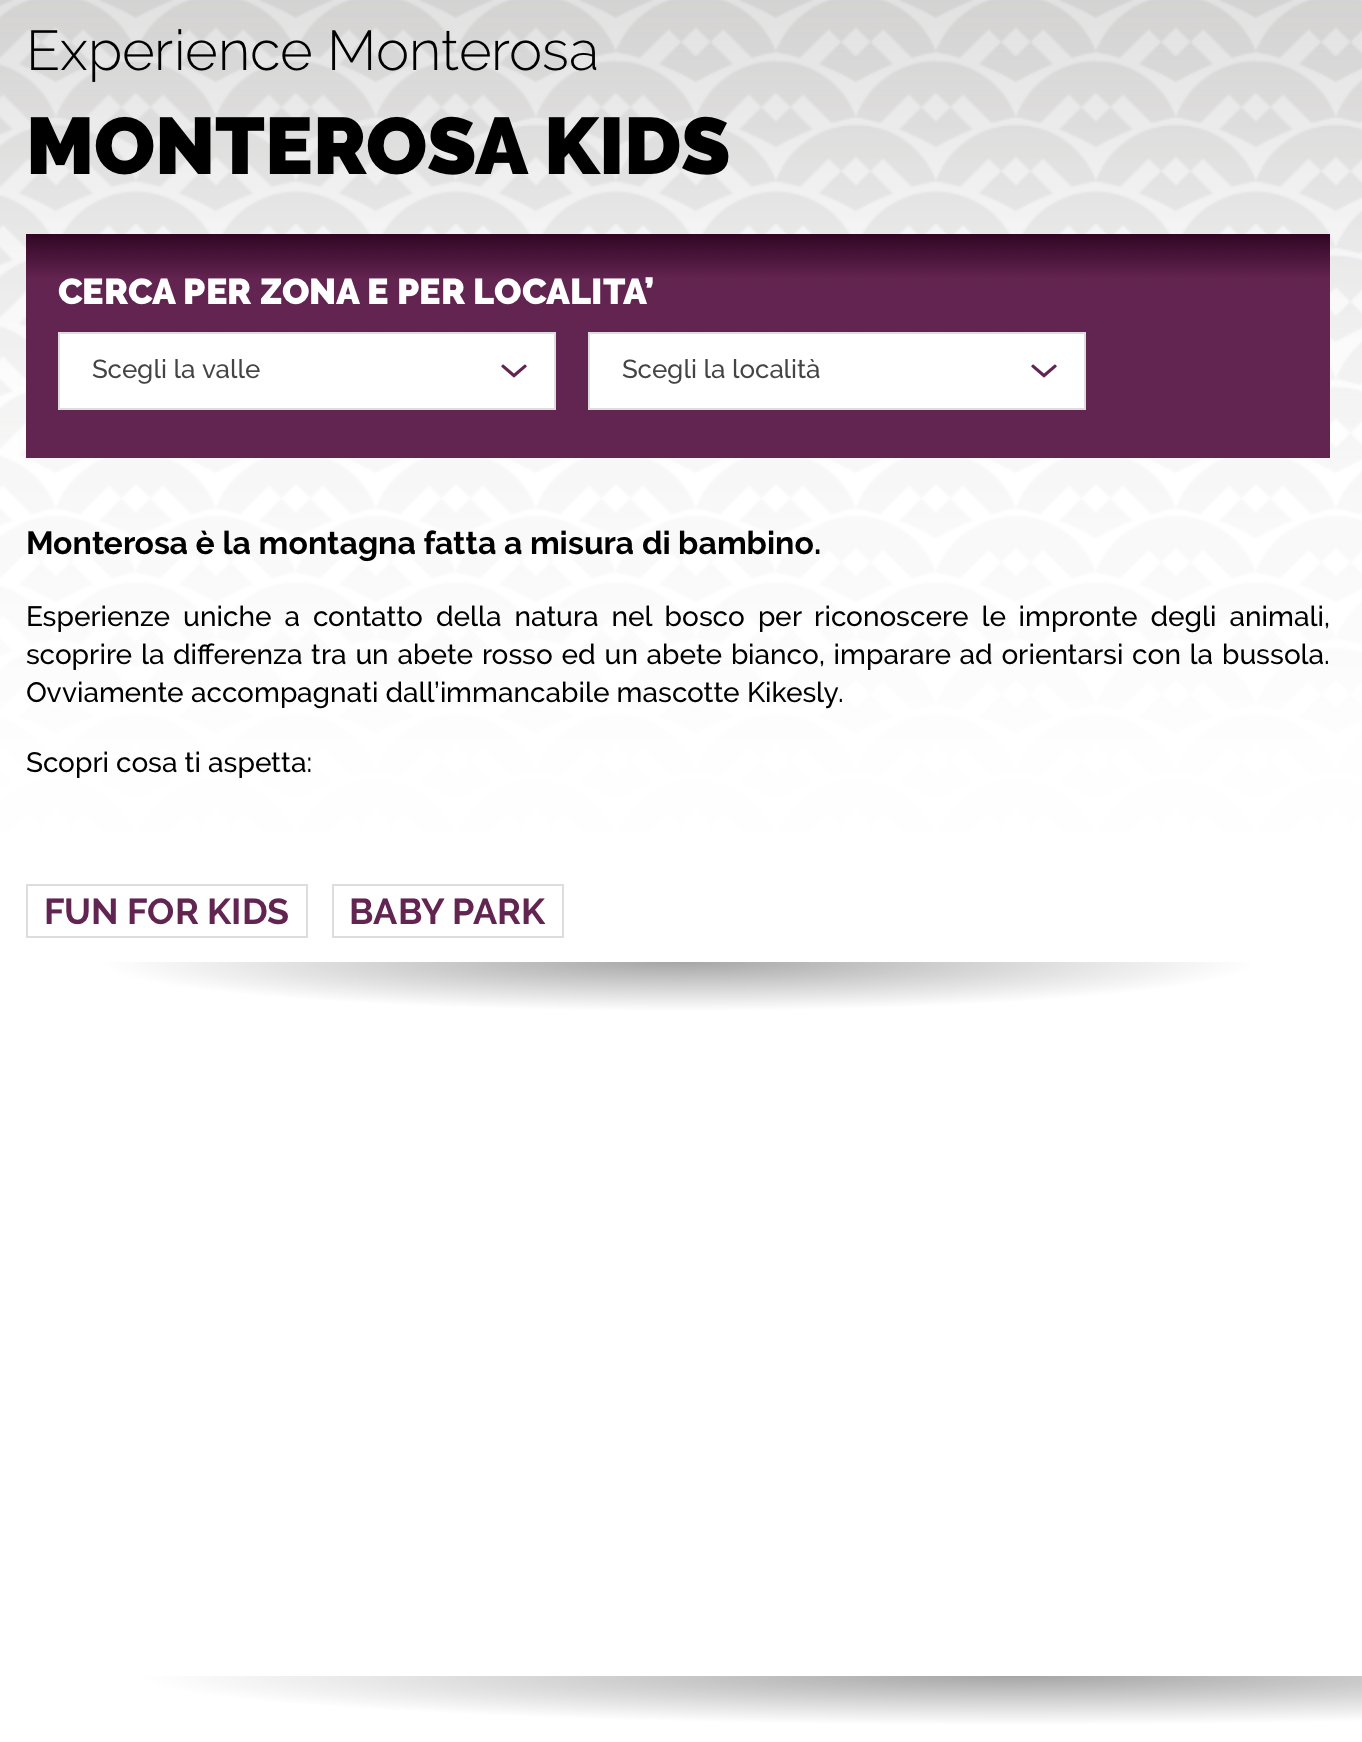
\includegraphics[width=1\linewidth, keepaspectratio]{12-interaction-consistency}
        \caption{\href{https://www.visitmonterosa.com/experience-monterosa/famigliare/}{link}.}
        \label{fig:interaction-consistency-02}
    \end{minipage} 
\end{figure}

\begin{figure}[H]
    \begin{minipage}[t]{0.5\textwidth}
        \centering
        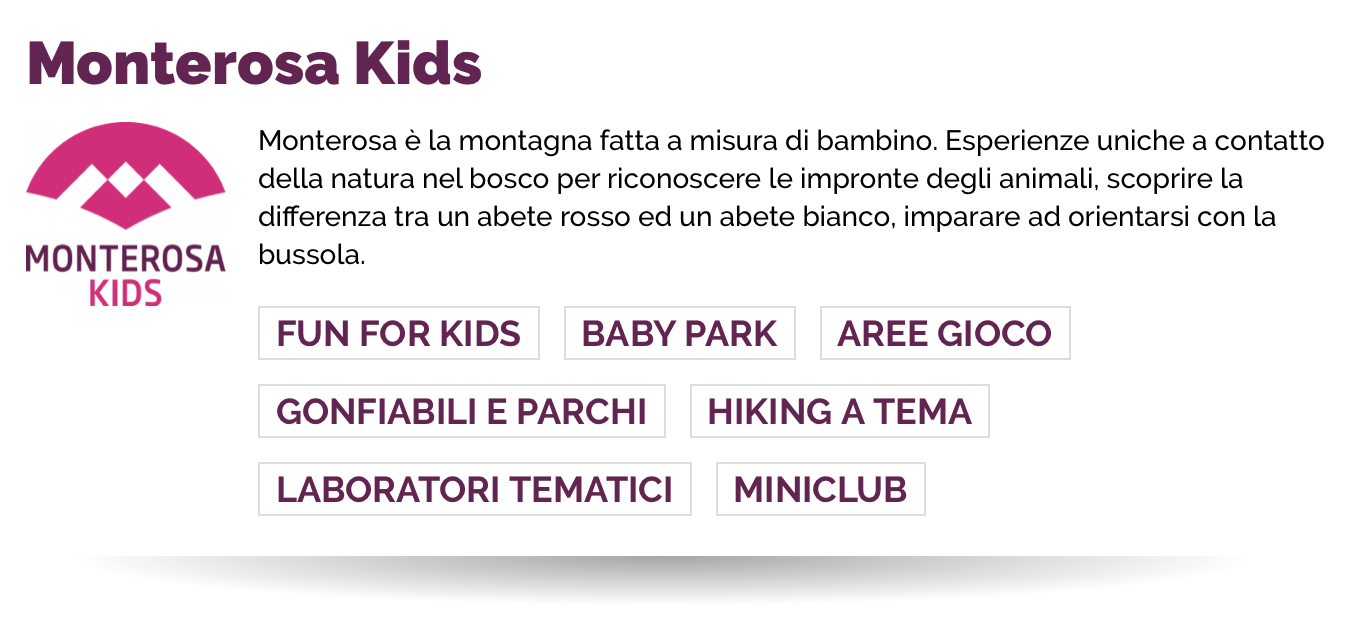
\includegraphics[width=1\linewidth, keepaspectratio]{13-interaction-consistency}
        \caption{\href{https://www.visitmonterosa.com/experience-monterosa/}{link}.}
        \label{fig:interaction-consistency-03}
    \end{minipage}   
    \hspace*{\fill}
    \begin{minipage}[t]{0.5\textwidth}
        \centering
        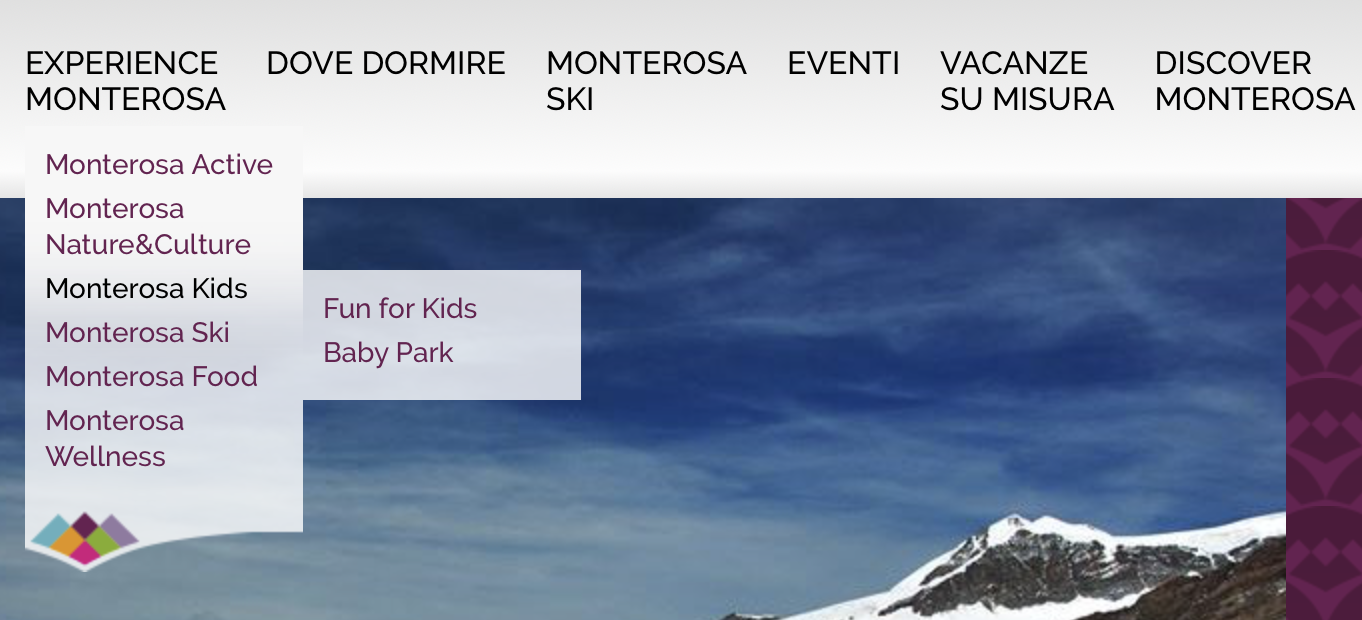
\includegraphics[width=1\linewidth, keepaspectratio]{14-interaction-consistency}
        \caption{\href{https://www.visitmonterosa.com}{link}.}
        \label{fig:interaction-consistency-04}
    \end{minipage} 
\end{figure}

\begin{figure}[H]
    \begin{minipage}[t]{0.5\textwidth}
        \centering
        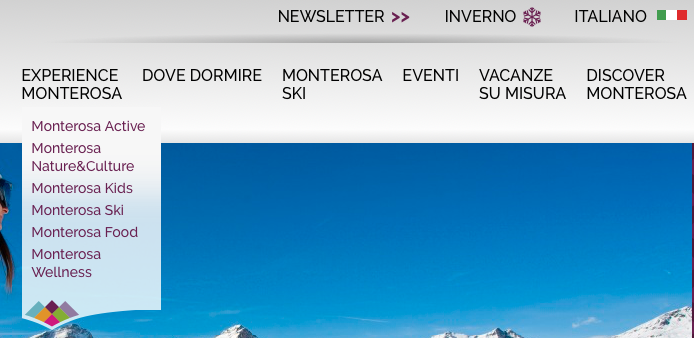
\includegraphics[width=1\linewidth, keepaspectratio]{15-interaction-consistency}
        \caption{\href{https://www.visitmonterosa.com}{link}.}
        \label{fig:interaction-consistency-05}
    \end{minipage}   
    \hspace*{\fill}
    \begin{minipage}[t]{0.5\textwidth}
        \centering
        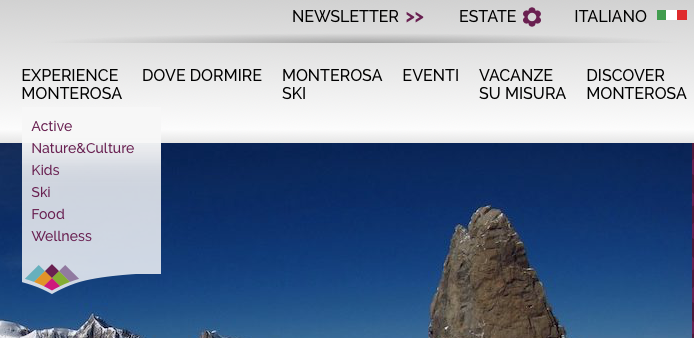
\includegraphics[width=1\linewidth, keepaspectratio]{16-interaction-consistency}
        \caption{\href{https://www.visitmonterosa.com/?season=summer}{link}.}
        \label{fig:interaction-consistency-06}
    \end{minipage} 
\end{figure}

\paragraph{Group navigation}
\begin{itemize}
    \item It is not possible to navigate among pages of the same group (e.g., among events).
    \item It is not possible to navigate from a specific page to a group main page unless through browser capabilities.
\end{itemize}

\paragraph{Structural navigation}
\begin{itemize}
    \item Because each topic is only made of text, the website does not present particular structural navigation problems.
\end{itemize}

\paragraph{Semantic navigation}
\begin{itemize}
    \item It is not possible to navigate from a topic to a related one (e.g., among events).
\end{itemize}

\paragraph{Landmarks}
\begin{itemize}
    \item The majority of landmarks fulfill their purpose.
    \item Newsletter as a landmark isn't useful to navigate the website.
\end{itemize}

\section{Content}

\paragraph{Information overload}
\begin{itemize}
    \item Even if some pages have more content than other, the information load is not overwhelming overall.
\end{itemize}

\section{Layout}

\paragraph{Text layout}
\begin{itemize}
    \item Not every paragraph is justified.
\end{itemize}

\paragraph{Interaction placeholder}
\begin{itemize}
    \item Some links are not immediately recognizable (Figure \ref{fig:interaction-placeholder-01}).
    \item Some buttons are used in place of labels (Figure \ref{fig:interaction-placeholder-02}).
\end{itemize}

\begin{figure}[H]
    \begin{minipage}[t]{0.5\textwidth}
        \centering
        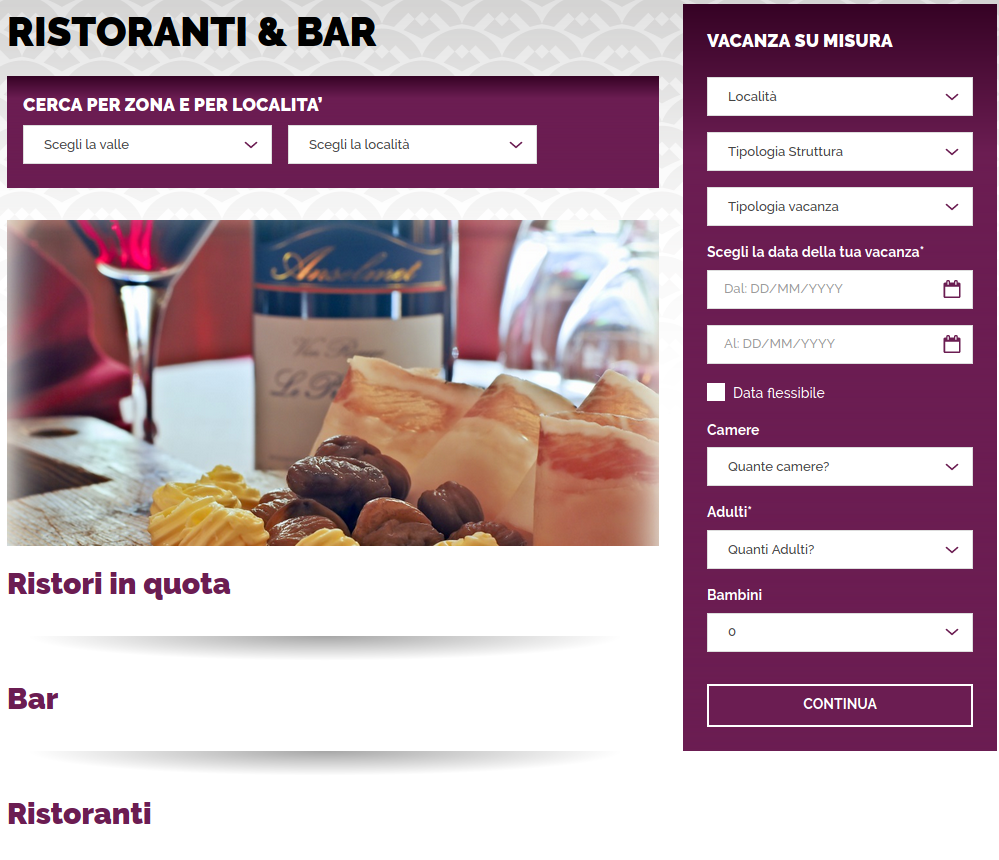
\includegraphics[width=1\linewidth, keepaspectratio]{81-interaction-placeholders-links}
        \caption{https://www.visitmonterosa.com/discover-monterosa/ristoranti-e-bar/}
        \label{fig:interaction-placeholder-01}
    \end{minipage}   
    \hspace*{\fill}
    \begin{minipage}[t]{0.5\textwidth}
        \centering
        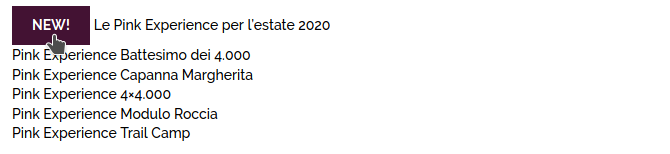
\includegraphics[width=1\linewidth, keepaspectratio]{82-interaction-placeholders-labels}
        \caption{https://www.visitmonterosa.com/monterosa-ski/monterosa-liberamente-femminile/}
        \label{fig:interaction-placeholder-02}
    \end{minipage} 
\end{figure}


\paragraph{Spatial allocation}
\begin{itemize}
	\item The search bar is placed on the bottom of the page, hence it is difficult to find. ((Figure \ref{fig:spatial-allocation-01}).)
\end{itemize}

\begin{figure}[H]
	\centering
	\begin{minipage}[t]{0.5\textwidth}
		\centering
		
\includegraphics[width=1\linewidth, keepaspectratio]{91-spatial-allocation-searchbar}
		\caption{https://www.visitmonterosa.com/}
		\label{fig:spatial-allocation-01}
	\end{minipage} 
\end{figure}


\paragraph{Consistency of page structure}
\begin{itemize}
	\item Some pages have a search bar or a "potrebbe interessarti" section, others don't. (Figure \ref{fig:consistency-01} and \ref{fig:consistency-02}).
    \item Some pages have missing images (Figure \ref{fig:consistency-03}).
\end{itemize}

\begin{figure}[H]
    \begin{minipage}[t]{0.5\textwidth}
        \centering
        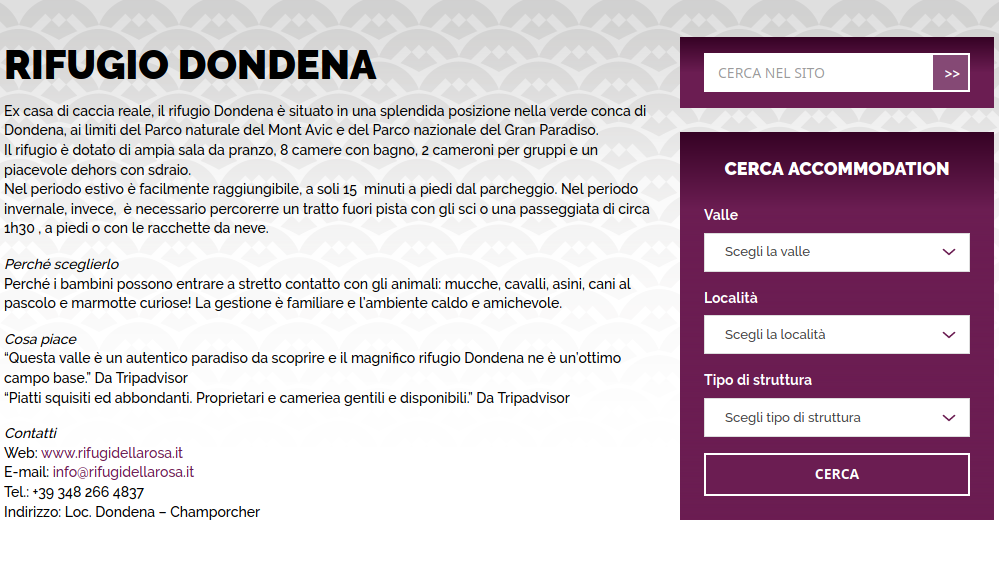
\includegraphics[width=1\linewidth, keepaspectratio]{101-consistency-missing-stuff}
        \caption{https://www.visitmonterosa.com/accommodation/rifugio-dondena/}
        \label{fig:consistency-01}
    \end{minipage}   
    \hspace*{\fill}
    \begin{minipage}[t]{0.5\textwidth}
        \centering
        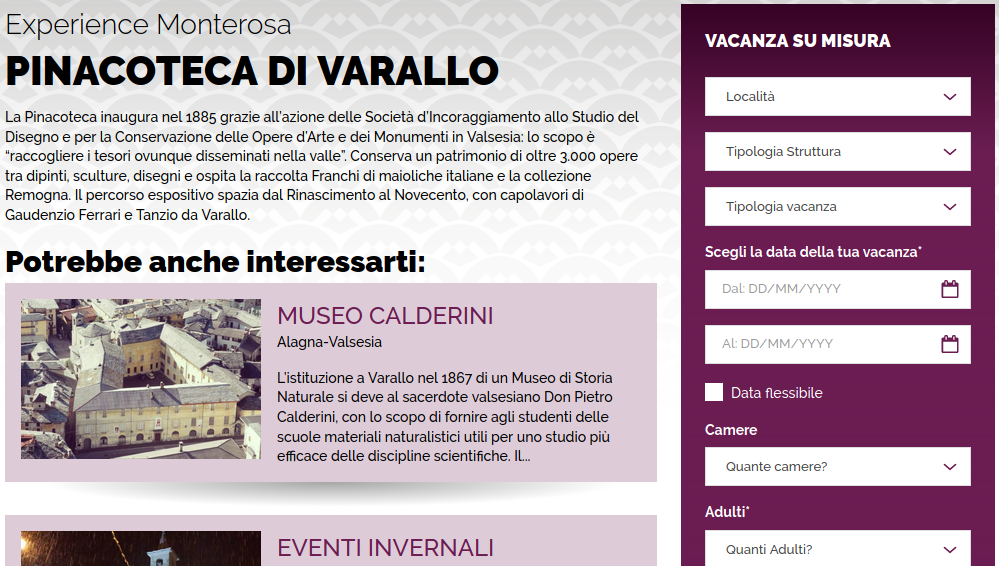
\includegraphics[width=1\linewidth, keepaspectratio]{102-consistency-missing-stuff}
        \caption{https://www.visitmonterosa.com/experience/pinacoteca-di-varallo/}
        \label{fig:consistency-02}
    \end{minipage} 
\end{figure}

\begin{figure}[H]
	\centering
	\begin{minipage}[t]{0.5\textwidth}
		\centering
		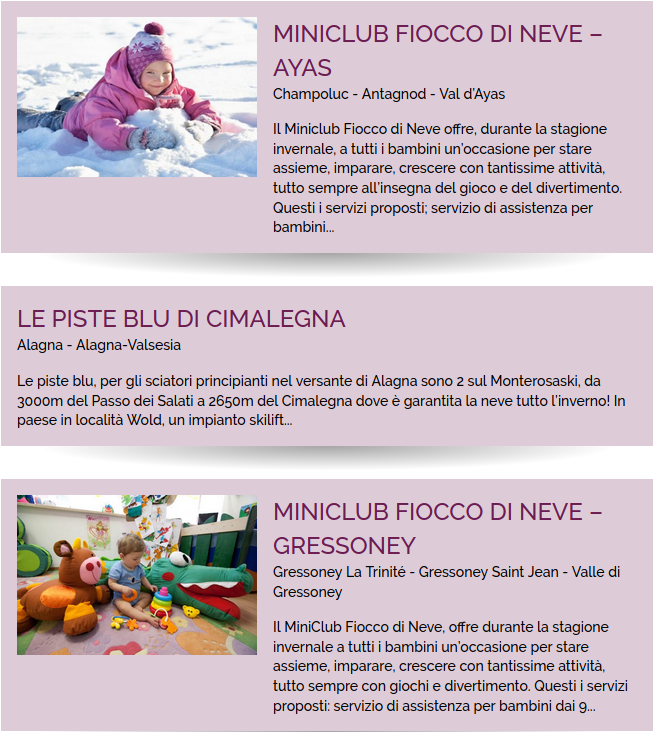
\includegraphics[width=1\linewidth, keepaspectratio]{103-consistency-missing-images}
		\caption{https://www.visitmonterosa.com/experience-monterosa/famigliare/fun-for-kids/}
		\label{fig:consistency-03}
	\end{minipage} 
\end{figure}


\chapter{Aggregated results and discussions}

% TODO: Aggregate data and visual representation

\chapter{Conclusion}

% TODO: todo





\end{document}
